%%%%%%%%%%%%%%%%%%%%%%%%%%%%%%%%
\section{Results} \label{S:results}
%%%%%%%%%%%%%%%%%%%%%%%%%%%%%%%%
%
%###############################
\subsection{About the hierarchy of variability} \label{sS:results_variability}
%###############################
%
As expected, three hierarchies of variability were present in our data: the blocks and children's random effects, as well as, the variability of the entropy replicates.

Evidence from the posterior estimates reveal the block random effects explained a small amount of variability in the data (top panel of figure \ref{fig:variability}), and its inclusion/exclusion in the model did not change the parameter estimates. The previous implies the experiment was correctly `set up', as the series in which the utterances were transcribed did not explain a significant amount of variation, nor its exclusion biased the parameter estimates.

On the contrary, we observe a significantly larger variability between children's \textit{speech intelligibility}, i.e. more than three times the block effects variability (middle panel of figure \ref{fig:variability}). The previous corroborated preliminary evidence on the matter \cite{Young_et_al_2002, Peng_et_al_2004, Montag_et_al_2014, Castellanos_et_al_2014, Yanbay_et_al_2014, Nittrouer_et_al_2014, Freeman_et_al_2017, Boonen_et_al_2021}. Additionally, it implied that given such a large amount of between variability, the statistical models might have a harder time comparing the two \textit{hearing status} groups, in respect to their location on the intelligibility scale.

Finally, for the variability of the entropy replicates, the posterior estimates provide a surprising finding: the amount of variability at the replicates level is even larger than the one observed at the children level (bottom panel of figure \ref{fig:variability}). The latter implies there is significant error in measuring speech intelligibility with multiple entropy replicates. This further emphasize the difficulty of producing unequivocal  inferences, in respect to the intelligibility levels of the \textit{hearing status} groups.
%
\begin{figure}[!h]
	\centering
	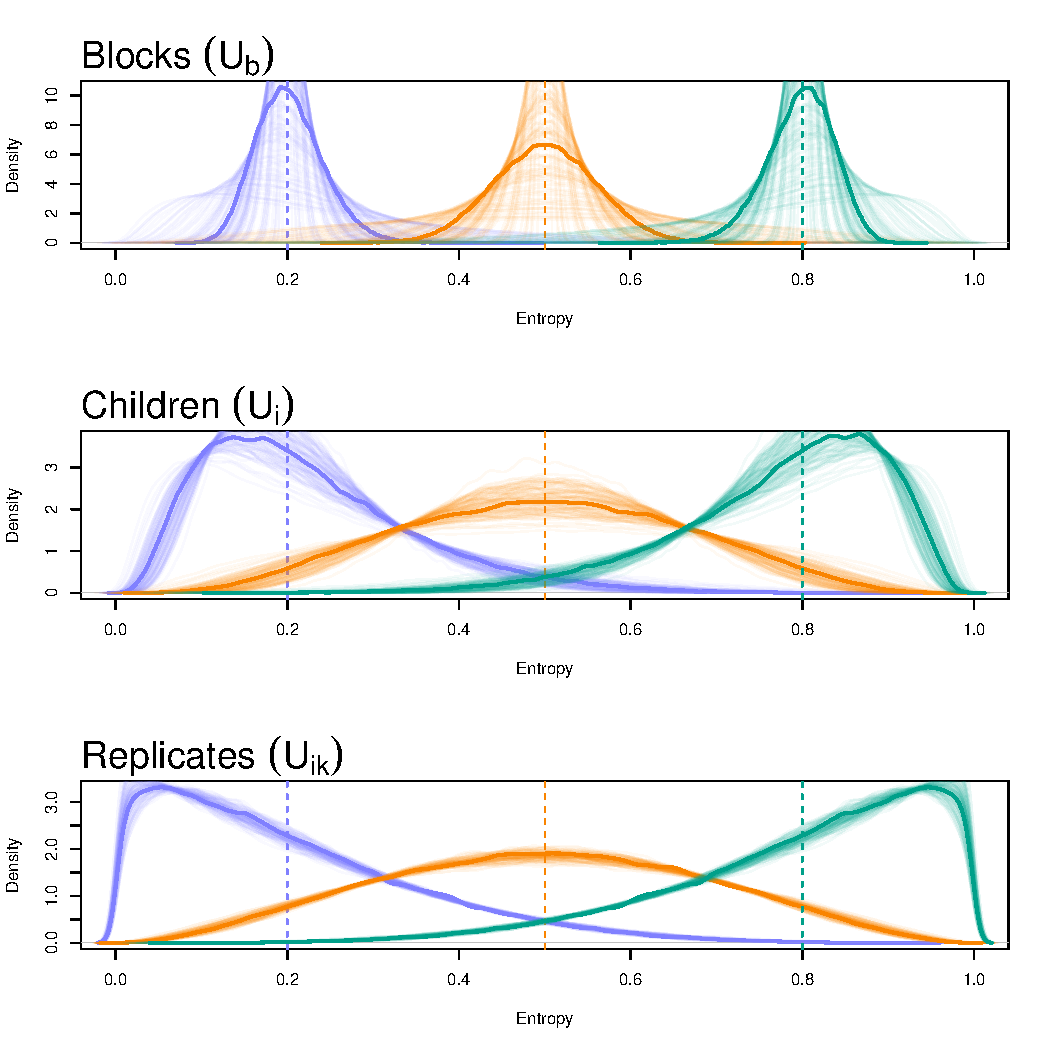
\includegraphics[width=0.5\linewidth]{variability_plot.pdf}
	\caption[Posterior predictive: hierarchy of variability in the data]{Posterior predictive: hierarchy of variability in the data. Distributions are plotted at entropy replicates' scale, considering three different average entropy values: $\mu=0.2$, $\mu=0.5$, and $\mu=0.8$ (discontinuous lines). }
	\label{fig:variability}
\end{figure}
%
%###############################
\subsection{About our hypothesis} \label{sS:results_hypothesis}
%###############################
%
The current research used the Information-Theoretic Approach \citep{Anderson_2008, Chamberlain_1965} for model selection and inference. The application of the approach required: (i) the expression of the research hypothesis into statistical models, (ii) the selection of the most plausible models, and (iii) to produce inferences based on one or multiple selected models.

Since the first requirement is covered in sections \ref{sS:causal_frame} and \ref{sS:stat_analysis}, and expanded in supplementary sections \ref{sSA:causal_details} and \ref{sSA:model_details}, while the second requirement is detailed in the supplementary section \ref{ssSA:model_selection}, here we proceed with the last step of the approach. 

Considering all of the above, the final inferences will be performed with models three and ten. The former is considered because it is the highest supported model. The latter is considered because it encompasses the remaining highest supported models. Furthermore, no \textit{robust} model is analyzed, as we prefer a more parsimonious depiction of our hypothesis.

\textcolor{red}{work in progress}

\begin{comment}
“simplest” model (E_NC2b) provides
(preliminar) evidence on,
the higher the unaided PTA the
lower the child’s SI (bP[2])
(based on power analysis, we can be
sure is a small effect)
no apparent statistical difference
between NH and HI=CI children
(but this requires a CONTRAST)
for each “hearing” year, the SI
increases in approx 0:40 logits
(effect larger than the assumed in
power analysis)


however, the “interaction” model
(E_NC5b3) shows similar results on,
the small (still non-significant)
effects of the unaided PTA on the
child’s SI
similar explained variability across
levels and blocks
(similar to the “simplest” model)
but “mild” evidence of prevalent
interactions,
SI means for HI=CI per E,
aEHS[2; 2] (Genetic) vs
aEHS[3; 2] (CMV)
different SI evolution for NH vs
HI=CI children, per unit A
(bAHS),

within the “interaction” model,
the size of the data within groups
from combinations of E and HS,
does not allow to reject the
contrasts’ null hypothesis,
similar result is observed on the
bAHS contrast
(because the effect is small, compared
to children’s variability)
but we still observe differences
between NH and HI/CI, and even
within HI/CI by E,
therefore we decide to keep the
(E_NC5b3) model
\end{comment}

\begin{comment}
It is important to highlight that for all model implementations, the visual inspection of trace, trace-rank and autocorrelation plots was performed. Additionally, we also evaluated the Gelman-Rubin diagnostic and effective number of samples \cite{Gelman_et_al_2014}. In all cases, the plots and statistics indicated the parameters achieved convergence, good mixing and lack of serial autocorrelation; all necessary requirements to be able to interpret the model estimates. 

Finally, considering the evidence provided by the previous step, we proceed to make inferences based on the selected models.
\end{comment}

\begin{comment}
	Following the successful and comprehensive analysis in \citet{vanDaal_2020} and \citet{Lesterhuis_2018}, 
	
	Notice the model depicted in panel (a) is interested on (what we can call) \textit{total effects}, i.e. the effects of the hearing characteristics, not independent from the effects of the hearing apparatus (cochlear implant or hearing aid). This is important to understand for two reasons. Since a hearing apparatus is fitted onto a child depending on aspects such as the locus and severity of his(her) hearing impairment \citep{Korver_et_al_2017}: (1) such specific children's characteristics could confound the (beneficial) effects of using specific hearing apparatuses, while (2) because children are selected from a convenient sample, not representative of their respective populations (see section \ref{s_sect:children}), the need to control for such characteristics is paramount, if we seek to obtain effects that can generalize better and beyond our sample\footnote{follow the \textit{notes} folder, to see a graphical though experiment.}.
	
	Considering the previous, we propose the model depicted in panel (b), where we control for the possible confounding variables etiology ($E_{i}$), \textcolor{blue}{as a proxy of locus}, and unaided PTA ($PTA_{i}$), as a proxy for hearing impairment severity. In that sense, the model would estimate (what we can call) the \textit{direct effects} of the hearing apparatus, independent of the children's characteristics.
\end{comment}
%
%
%###############################
\subsection{The speech intelligibility scale} \label{sS:results_scales}
%###############################
%
\textcolor{red}{work in progress}
%
\begin{figure}[!h]
	\centering
	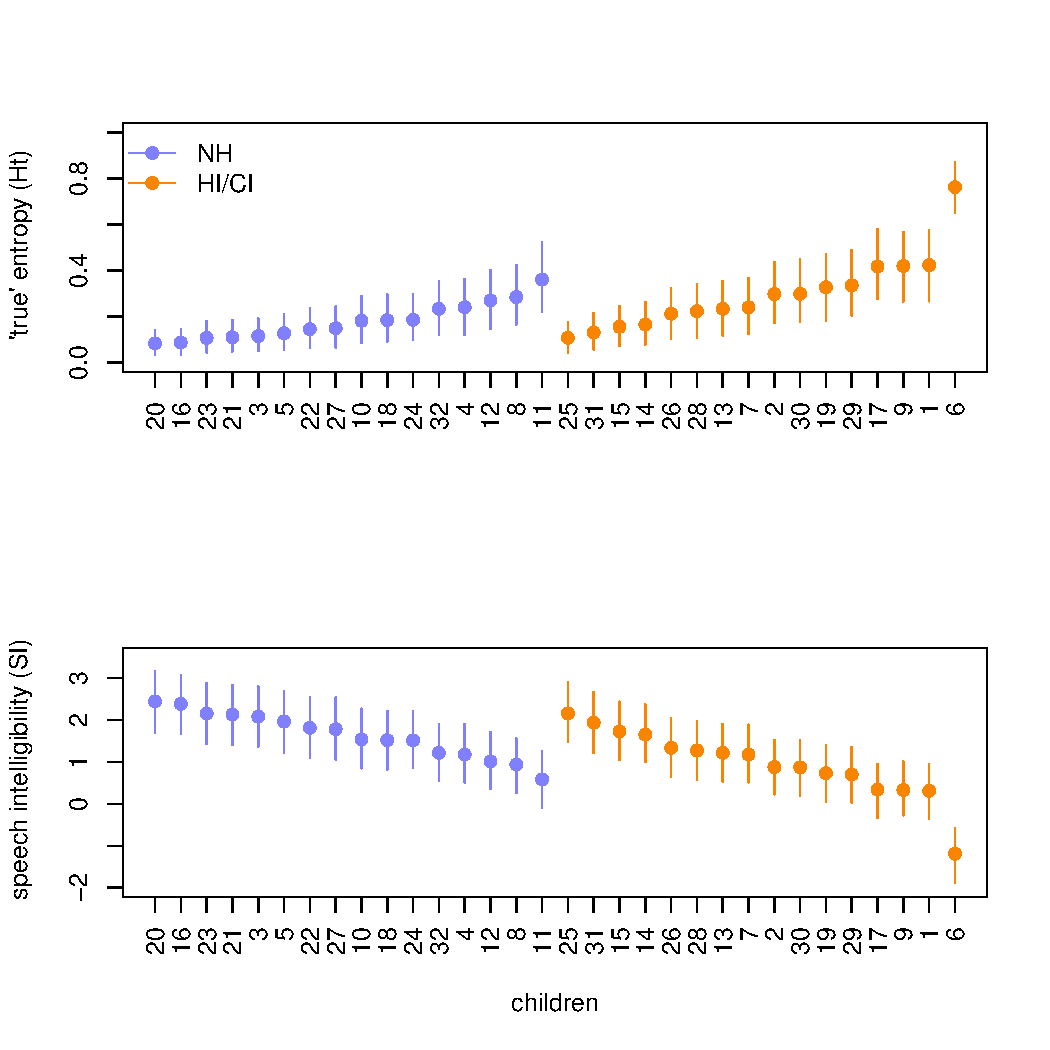
\includegraphics[width=0.7\linewidth]{posterior_predictive_real2.pdf}
	\caption[Posterior predictive: ``true'' entropy and intelligibility scales]{Posterior predictive: ``true'' entropy and speech intelligibility scales}
	\label{fig:predictive2}
\end{figure}
%
%
%###############################
\subsection{Posterior predictive} \label{sS:results_posterior}
%###############################
%
\textcolor{red}{work in progress}
%
\begin{figure}[!h]
	\centering
	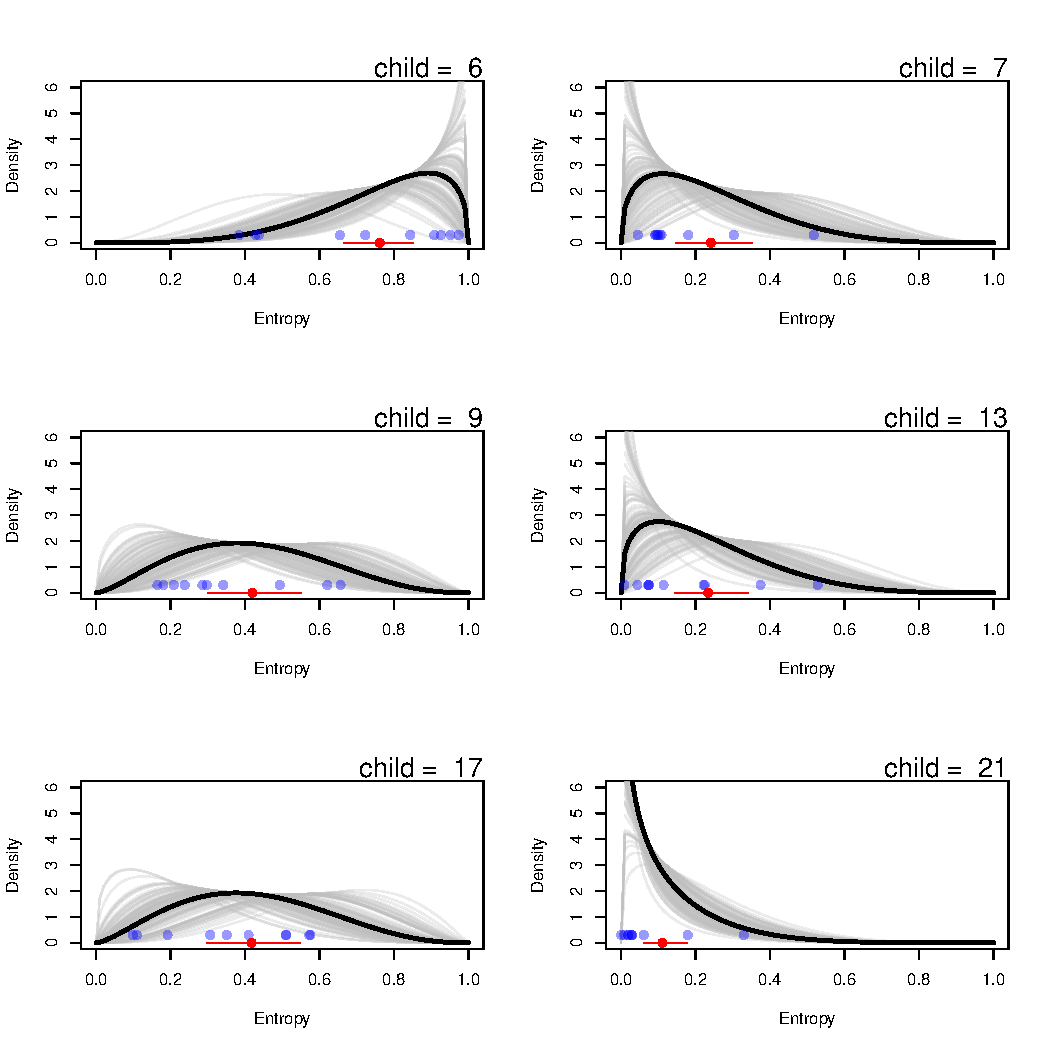
\includegraphics[width=0.7\linewidth]{posterior_predictive_real1.pdf}
	\caption[Posterior predictive: entropy replicates]{Posterior predictive: entropy replicates}
	\label{fig:predictive1}
\end{figure}
%
%
%###############################
\subsection{Outlying observations} \label{sS:results_outliers}
%###############################
%
\textcolor{red}{work in progress}
%
\begin{figure}[!h]
	\centering
	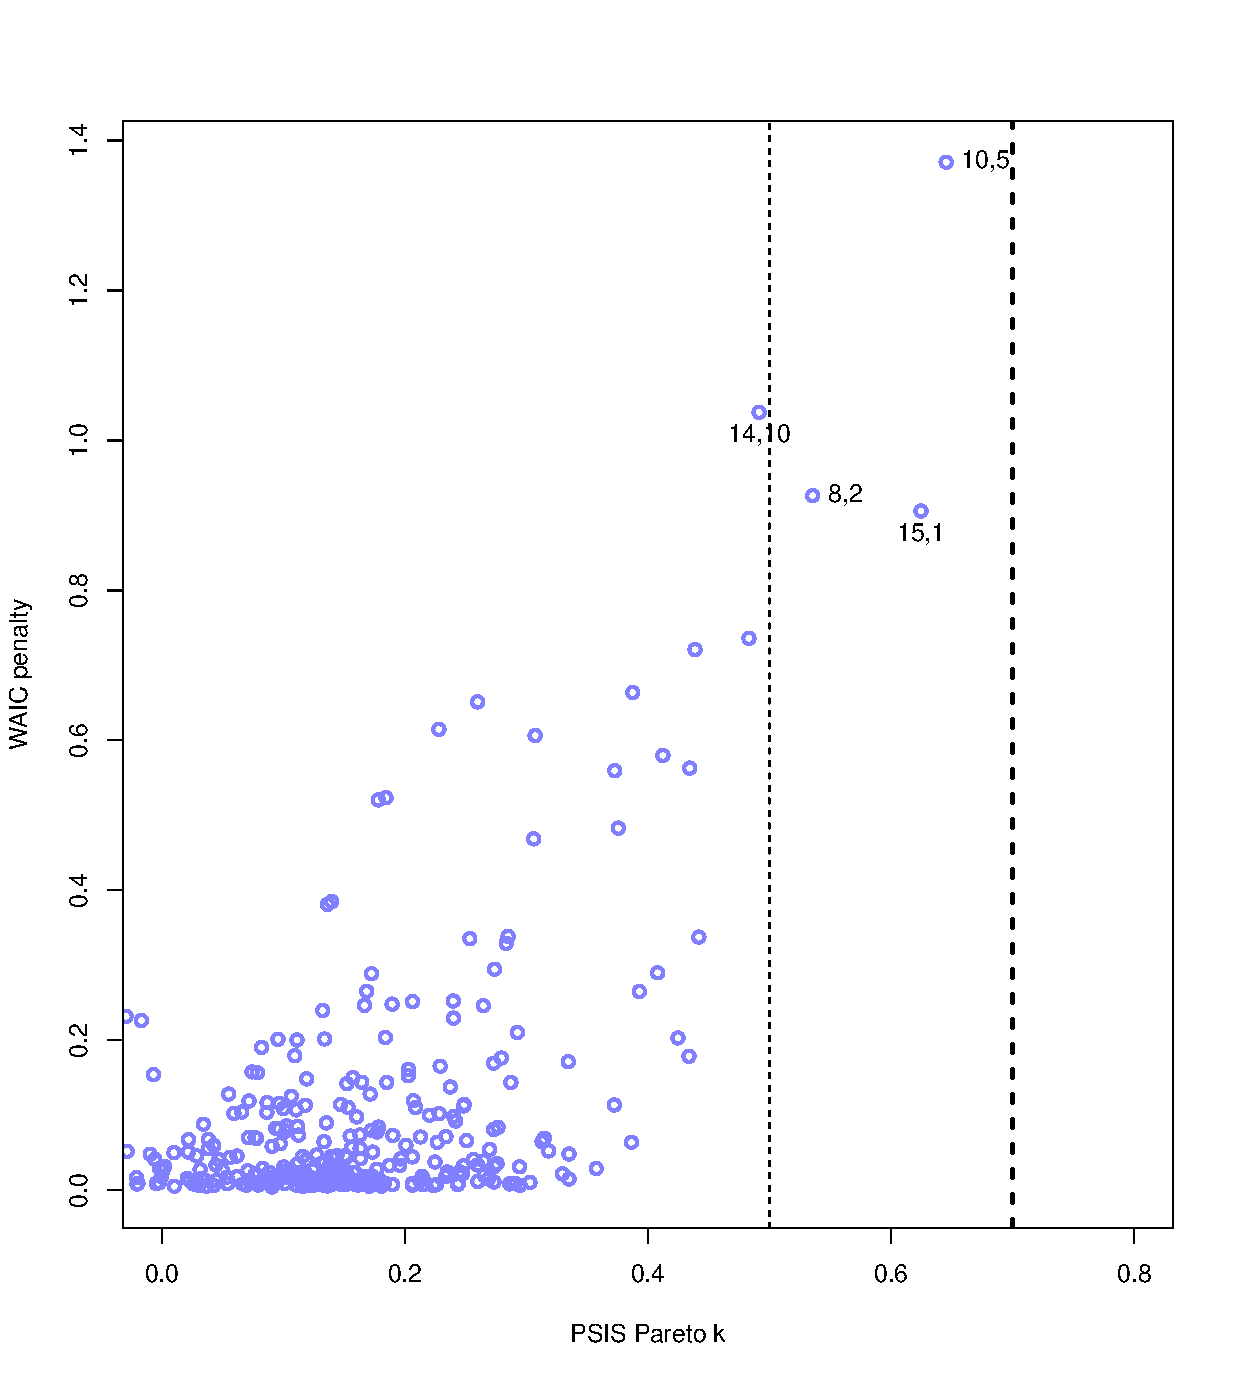
\includegraphics[width=0.5\linewidth]{outliers.pdf}
	\caption[Outlying observations]{Outlying observations. Pairs (child, utterance) are reported for specific observations.}
	\label{fig:outliers}
\end{figure}
%
%